\documentclass[12pt]{article}

\usepackage{amsmath, amsthm, ulem, graphicx, marvosym, fancyhdr, amscd, amssymb, mathrsfs,color,subcaption,nicefrac,hyperref}
\usepackage{framed}
\usepackage{tikz}
\usepackage{showkeys}

\newcommand\Z{{\mathbb Z}}
\newcommand\F{{\mathbb F}}
\newcommand\N{{\mathbb N}}
\newcommand\bE{{\mathbf E}}
\newcommand\p{{\mathscr P}}
\newcommand\R{{\mathbb R}}
\newcommand\Q{{\mathbb Q}}

\topmargin -.5in
\evensidemargin-.3in
\oddsidemargin-.3in
\textheight 9.5in
\textwidth 7in

\newtheorem*{theorem}{Theorem}
\newtheorem{lemma}{Lemma}
\newtheorem{prop}{Proposition}
\newtheorem{cor}{Corollary}


%\setlength{\voffset}{-1in}

\everymath={\displaystyle}

%%% 
% Framed mini-page environment 
%%%
\newsavebox{\fmbox}
   \newenvironment{ans}
     {\begin{lrbox}{\fmbox}\begin{minipage}{13cm} \textbf{Answer:} \par}
     {\end{minipage}\end{lrbox}\fbox{\usebox{\fmbox}} \vspace{0.25cm}}

\newcommand{\lcm}{\operatorname{lcm}}
\newcommand{\ds}{\displaystyle}

%\pagestyle{fancy}

\renewcommand{\headrulewidth}{0pt}
%\rhead{}
%\lhead{}
%\cfoot{\Huge\Stopsign}

\pagestyle{empty}

\title{Tree Power Notes}


\author{author\thanks{University of Washington, Tacoma, WA} %\and author\thanks{institue2} 
\and author\footnotemark[1]}

\begin{document}

\maketitle

\noindent ABSTRACT. 

\vspace{1cm}

\noindent Key words: 


\section*{Introduction}  \textcolor{red}{Literature review:}



\section{Assumptions}

With these assumptions, the DE problem reduces to 1D.
\begin{enumerate}
\item We assume all trees we consider are roughly the same. That means same height, same radius
\item With the previous assumption, we place all devices at the same height, and same depth
\end{enumerate}

\section{To do (Feb 7)}
Our goal is to write Python scripts that would simulate the temperature distribution in the trunk of the tree and the ambient environment. We will use the heat model for both. See the following reference for more detail:
\begin{enumerate}
\item Within a tree stem: see [\ref{heat}]
\item Ambient temperature: see [\ref{airtempforest}] and [\ref{evergreen}]
\end{enumerate}

\subsection{FD model of temperature within a tree stem}

Notations: 
\begin{enumerate}
\item $T$: temperature (K)
\item $\rho$: density (kg/m$^3$)
\item $c$: specific heat (J/(kgK))
\item $t$: time (s)
\item $k$: thermal conductivity (W/(mK))
\item $r$: distance from center of the tree (m)
\item $\phi$: azimuth angle, measured clockwise with south being $\phi=0$ (radian/degree), [\ref{heat}] assumes $\partial k/\partial \phi=0$
\item $\alpha$: albedo of the surface
\end{enumerate}

The basic heat equation for temperature distribution is 
\begin{equation}
\rho c\frac{\partial T}{\partial t}=\nabla\cdot(k\nabla T)=\frac{1}{r}\frac{\partial}{\partial r}\bigg(kr\frac{\partial T}{\partial r}\bigg)+\frac{1}{r}\frac{\partial}{\partial \phi}\bigg(\frac{k}{r}\frac{\partial T}{\partial \phi}\bigg)
\end{equation}

We add source terms for the diffusion equation to obtain
\begin{equation}
\rho c\frac{\partial T}{\partial t}=\nabla\cdot(k\nabla T)-\frac{1}{\Delta r}[H+(1-\alpha)(S_{dir}+S_{dif})+(IR_{in}-IR_{out})]
\end{equation}

In the following, we explain the source terms: 
\begin{enumerate}
\item 
Free convective heat loss/gain happens when the tree surface temp is different from the ambient temp. Forced convection happens when there is wind. We denote the heat loss/gain by $H$, and 
\begin{equation}
H=h(T_{sfc}-T_{air}),
\end{equation}
with $h$ (W/($m^2$K)) being the convective heat transfer coefficient. Here
\begin{equation}
h=h_{free}-h_{forced},
\end{equation}
more details in \ref{heat}. 

\item $S_{dir}+S_{dif}$ represents direct solar radiation, plus diffusion solar radiation. 

\item $IR_{in}-IR_{out}$ represents wave radiation from and to the tree. More details see [\ref{heat}].

\end{enumerate}

Our goal now is to solve this 2D differential equation with FD scheme.

\textcolor{red}{ref, see section 3.6: https://link.springer.com/content/pdf/10.1007\%2F978-3-319-55456-3.pdf} and

\textcolor{red}{https://pycav.readthedocs.io/en/latest/api/pde/crank\_nicolson.html}

\subsection{FD model of temperature in the forest}

To do.


\newpage

\section{To do (Jan 31)}
\begin{enumerate}
\item (DISCUSSION ITEM) Understand the hardware more: which equations to use, heat? thermoelectric? both? \textcolor{blue}{DONE. use heat equation. Goal is to model the temp in the tree and in the environment. At a same height. see\ref{sapwood}.}

\item (ACTION ITEM) Write code (Matlab/Python) to solve equations (equations see next section). \textcolor{red}{ref: http://www.claudiobellei.com/2016/11/10/crank-nicolson/}

\textcolor{red}{http://www.claudiobellei.com/2016/10/15/explicit-parabolic/}

\textcolor{blue}{1D code. Keep code in github repo: https://github.com/yajuna/treeRemote}

\item Verify the assumptions. 
\begin{enumerate}
\item With vertical drilling and data collection, find the best height. Call $h_0$\textcolor{blue}{see \ref{sapwood}}
\item With horizontal drilling and data collection, find the best depth. Call $r_0$
\end{enumerate}

With the assumption that we have found the ``best" height and radius (best: highest voltage, most activities, depending on the device??), we simplify the problem into a 1D problem. 


\item Find appropriate parameters in DE. For now, we take simple ones. \textcolor{red}{ISSUE: if real parameters are small or have varying magnitudes, might cause unexpected numerical errors}\textcolor{blue}{Waiting for confirmation from Nick.}


\end{enumerate}

\section{Differential Equations}

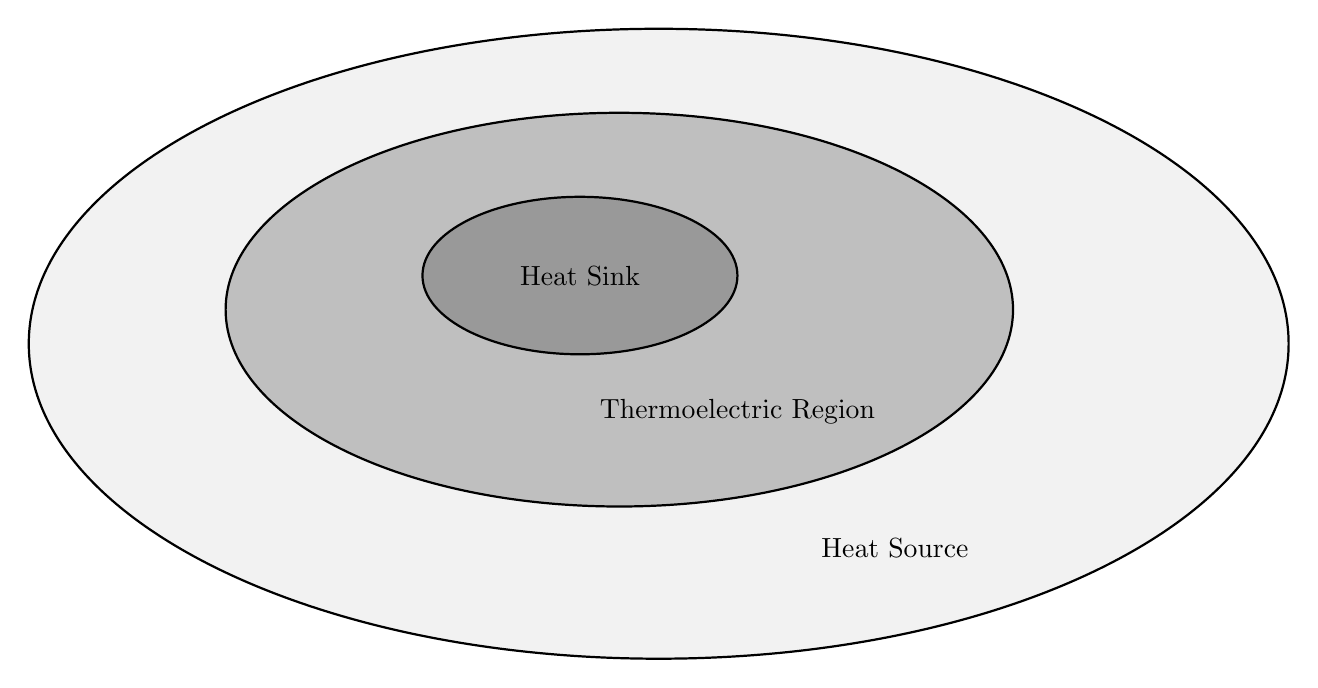
\begin{tikzpicture}
\def\angle{60}%
\pgfmathsetlengthmacro{\xoff}{2cm*cos(\angle)}%
\pgfmathsetlengthmacro{\yoff}{1cm*sin(\angle)}%
\draw [thick, fill=gray!10] (\xoff,-\yoff) circle[x radius=8cm, y radius=4cm] ++(3*\xoff,-3*\yoff) node{Heat Source};
\draw [thick, fill=gray!50] (0.5*\xoff,-0.5*\yoff) circle[x radius=5cm, y radius=2.5cm] ++(1.5*\xoff,-1.5*\yoff) node{Thermoelectric Region};
\draw [thick, fill=gray!80] (0,0) circle[x radius=2cm, y radius=1cm] node{Heat Sink};
\end{tikzpicture}

%ref for tikz: https://tex.stackexchange.com/questions/495446/drawing-concentric-ellipses-with-text-with-tikz

We modify the equations from [\ref{thermoelectric}], to radial equations.
Heat source and thermoelectric material in Fig.2[\ref{thermoelectric}] is now along the radius $r$. (\textcolor{red}{ASK ABOUT HARDWARE. Fig.1, and Fig.2. from ref})

Heat sink and resource for region $R$ are governed by the heat equation
\begin{equation}
\rho_R\ C_{vR}\ \frac{\partial T}{\partial t}=\nabla\cdot (k_R\nabla T),\label{heat}
\end{equation}

here, $T$ is the temperature, $t$ time, $\rho_R$ the density for region $R$, $C_{vR}$ specific heat, $k_R$ is the thermal conductivity. 

The middle layer is the thermoelectric region, governed by 
\begin{align}
\rho_{m}\ C_{vm}\ \frac{\partial T}{\partial t}&=\sigma\bE\cdot\bE-\sigma\cdot \alpha\bE\cdot \nabla T+\nabla\cdot[(k_m+\sigma\alpha^2T)\nabla T-\sigma\alpha T\bE],\label{elec}\\
\frac{\partial \rho}{\partial t}&=\nabla\cdot (-\sigma\bE+\sigma\alpha\nabla T).\label{chargedensity}
\end{align}
Here $\bE$ is the electric field, $\rho$ the charge density, $\sigma$ the electric conductivity, and $\alpha$ the Seebeck coefficient (\textcolor{red}{with temp dependence $\alpha=\alpha(T)$. Need curve fitting to decide}). 

\textcolor{red}{DO NOT KNOW ANY PARAMETERS}

\subsection{Reduction to 1D problem}
Based on our assumptions, we reduce spatial dependence to only on radius $r$: 
\begin{align}
\rho_R\ C_{vR}\ \frac{\partial T}{\partial t}&=\frac{\partial }{\partial r}\big(k_R\frac{\partial T}{\partial r}\big),\label{heat1d}\\
\rho_{m}\ C_{vm}\ \frac{\partial T}{\partial t}&=\sigma E^2-\sigma \alpha E\cdot \frac{\partial T}{\partial r}+\frac{\partial }{\partial r}[(k_m+\sigma\alpha^2T)\frac{\partial T}{\partial r}-\sigma\alpha T E],\label{elec1d}\\
\epsilon\frac{\partial E}{\partial t}&=J_0-\sigma E+\sigma\alpha\frac{\partial T}{\partial r}.\label{chargedensity1d}
\end{align}

Here \eqref{chargedensity1d} is the result of integrating \eqref{chargedensity}, and $J_0$ a constant. 

\subsection{Radial boundary conditions}

From outside inwards, the boundary conditions are:
\begin{itemize}
\item Outside: tree bark has $T_{amb}$.
\item Between Heat Source and Thermoelectric region, a voltage $V_0$ is generated, \textcolor{red}{heat flux and temperature??}
\item \textcolor{red}{section A. in Yan paper}

\end{itemize}

\newpage
Reference\textcolor{red}{BAD FORMAT. FOR convience only}
\begin{enumerate}
%%%%%%%%%%%% A
\item Yan. D. et al, Time-Dependent Finite-Volume Model of Thermoelectric Devices, IEEE, Transactions on industry applications, Vol. 50, No.1, Jan/Feb 2014\label{thermoelectric}

\item MIT notes online\label{mit}

\item Potter, A., Andresen, J., A finite-difference model of temperatures and heat flow within a tree stem, Can. J. For. Res. \textbf{32}, 548-555 (2002)\label{heat}

\item Bownman, W. et al, Sapwood temperature gradients between lower stems and the crown do not influence estimate of stand-level stem CO$_2$ efflux, Tree Physiology, 28, 1553-1559\label{sapwood}

\item Chen, J., et al, An empirical model for predictin diurnal air-temperature gradients from edge into old-growth Douglas-fir forest, Ecological Modeling, Vol. 67, Issues 2-4, pg 179-198, June 1993\label{airtempforest}

\item Tanja, S. et al., Air temperature triggers the recovery of evergreen boreal forest photosynthesis in spring, Global Change Biology, vol 9, issue 10, pg 1410-1426, Oct 2003\label{evergreen}

\end{enumerate}




\end{document}
